% !TEX root = diplomarbeit.tex
\chapter{Kommunikation Applikation und Hexacopter}
\renewcommand{\kapitelautor}{Autor: Katharina Joksch, Lucas Ullrich}
Um zwischen dem Hexacopter und dem Server eine Verbindung herzustellen wird eine Kommunikationsschnittstelle benötigt. Diese muss Drahtlos arbeiten und einen größeren Bereich
abdecken. Über diese werden anschließend die diversen Daten übertragen, dazu zählen \zB die Route, \bzw der Name des Gastes.

%%%%%%%%%%%%%%%%%%%%%%%%%%%%%%%%%%%%%%%%%%%%%%%%%%%%%%%%%%%%%%%%%%%%%%%%%%%%%%%
\section{Allgemeine technische Planung}
In der Planung wurde eine unkomplizierte und verlässliche Lösung für beide Kommunikationspartner gesucht. Da Bluetooth kaum noch standardmäßig verbaut wird hier wiederum
Serverseitig eine externe Hardware benötigt, um dies zu vermeiden wurde WLAN ins Auge gefasst.

WLAN stellte sich folglich als ideale Schnittstelle heraus,
es gibt die Möglichkeit zu Handover in sehr großen Bereichen, es ist nach einmaligem Setup vergleichsweise unkompliziert und es bietet diverse Möglichkeiten um festzustellen
ob die Verbindung noch aufrecht ist.

%%%%%%%%%%%%%%%%%%%%%%%%%%%%%%%%%%%%%%%%%%%%%%%%%%%%%%%%%%%%%%%%%%%%%%%%%%%%%%%
\section{Schnittstelle Hexacopter}
Seitens des Hexacopters wird ein zusätzliches Modul benötigt, dieses muss über eine der Schnittstellen des Mikrocontrollers ansprechbar sein.

  \subsection{Technische Planung}
  Bei der Planung wurde darauf geachtet ein WLAN-Modul zu wählen welches bekannter maßen funktioniert \bzw ein entsprechender Support zur Verfügung steht.
  So fiel die Wahl auf das WLAN-Modul RN171, vertrieben durch Microchip, hergestellt von Roving Networks.

  Das gewählte WLAN-Modul wird über eine UART-Schnittstelle angesteuert und verfügt über einige frei konfigurierbare Pins, diese werden schließlich zum Überwachen der
  Verbindung verwendet.

  \subsection{Umsetzung}
  Bei der Umsetzung stand für die anfänglichen Tests ein Evaluation-Kit zur Verfügung. Dieses kann ohne weitere Hardware direkt über ein USB-Kabel mit einem PC verbunden werden.
  So ist es möglich die nötigen Konfigurationen des Moduls auszutesten bevor dieses in der Hardware implementiert wird.

  \begin{figure}[tbh]
    \begin{centering}
      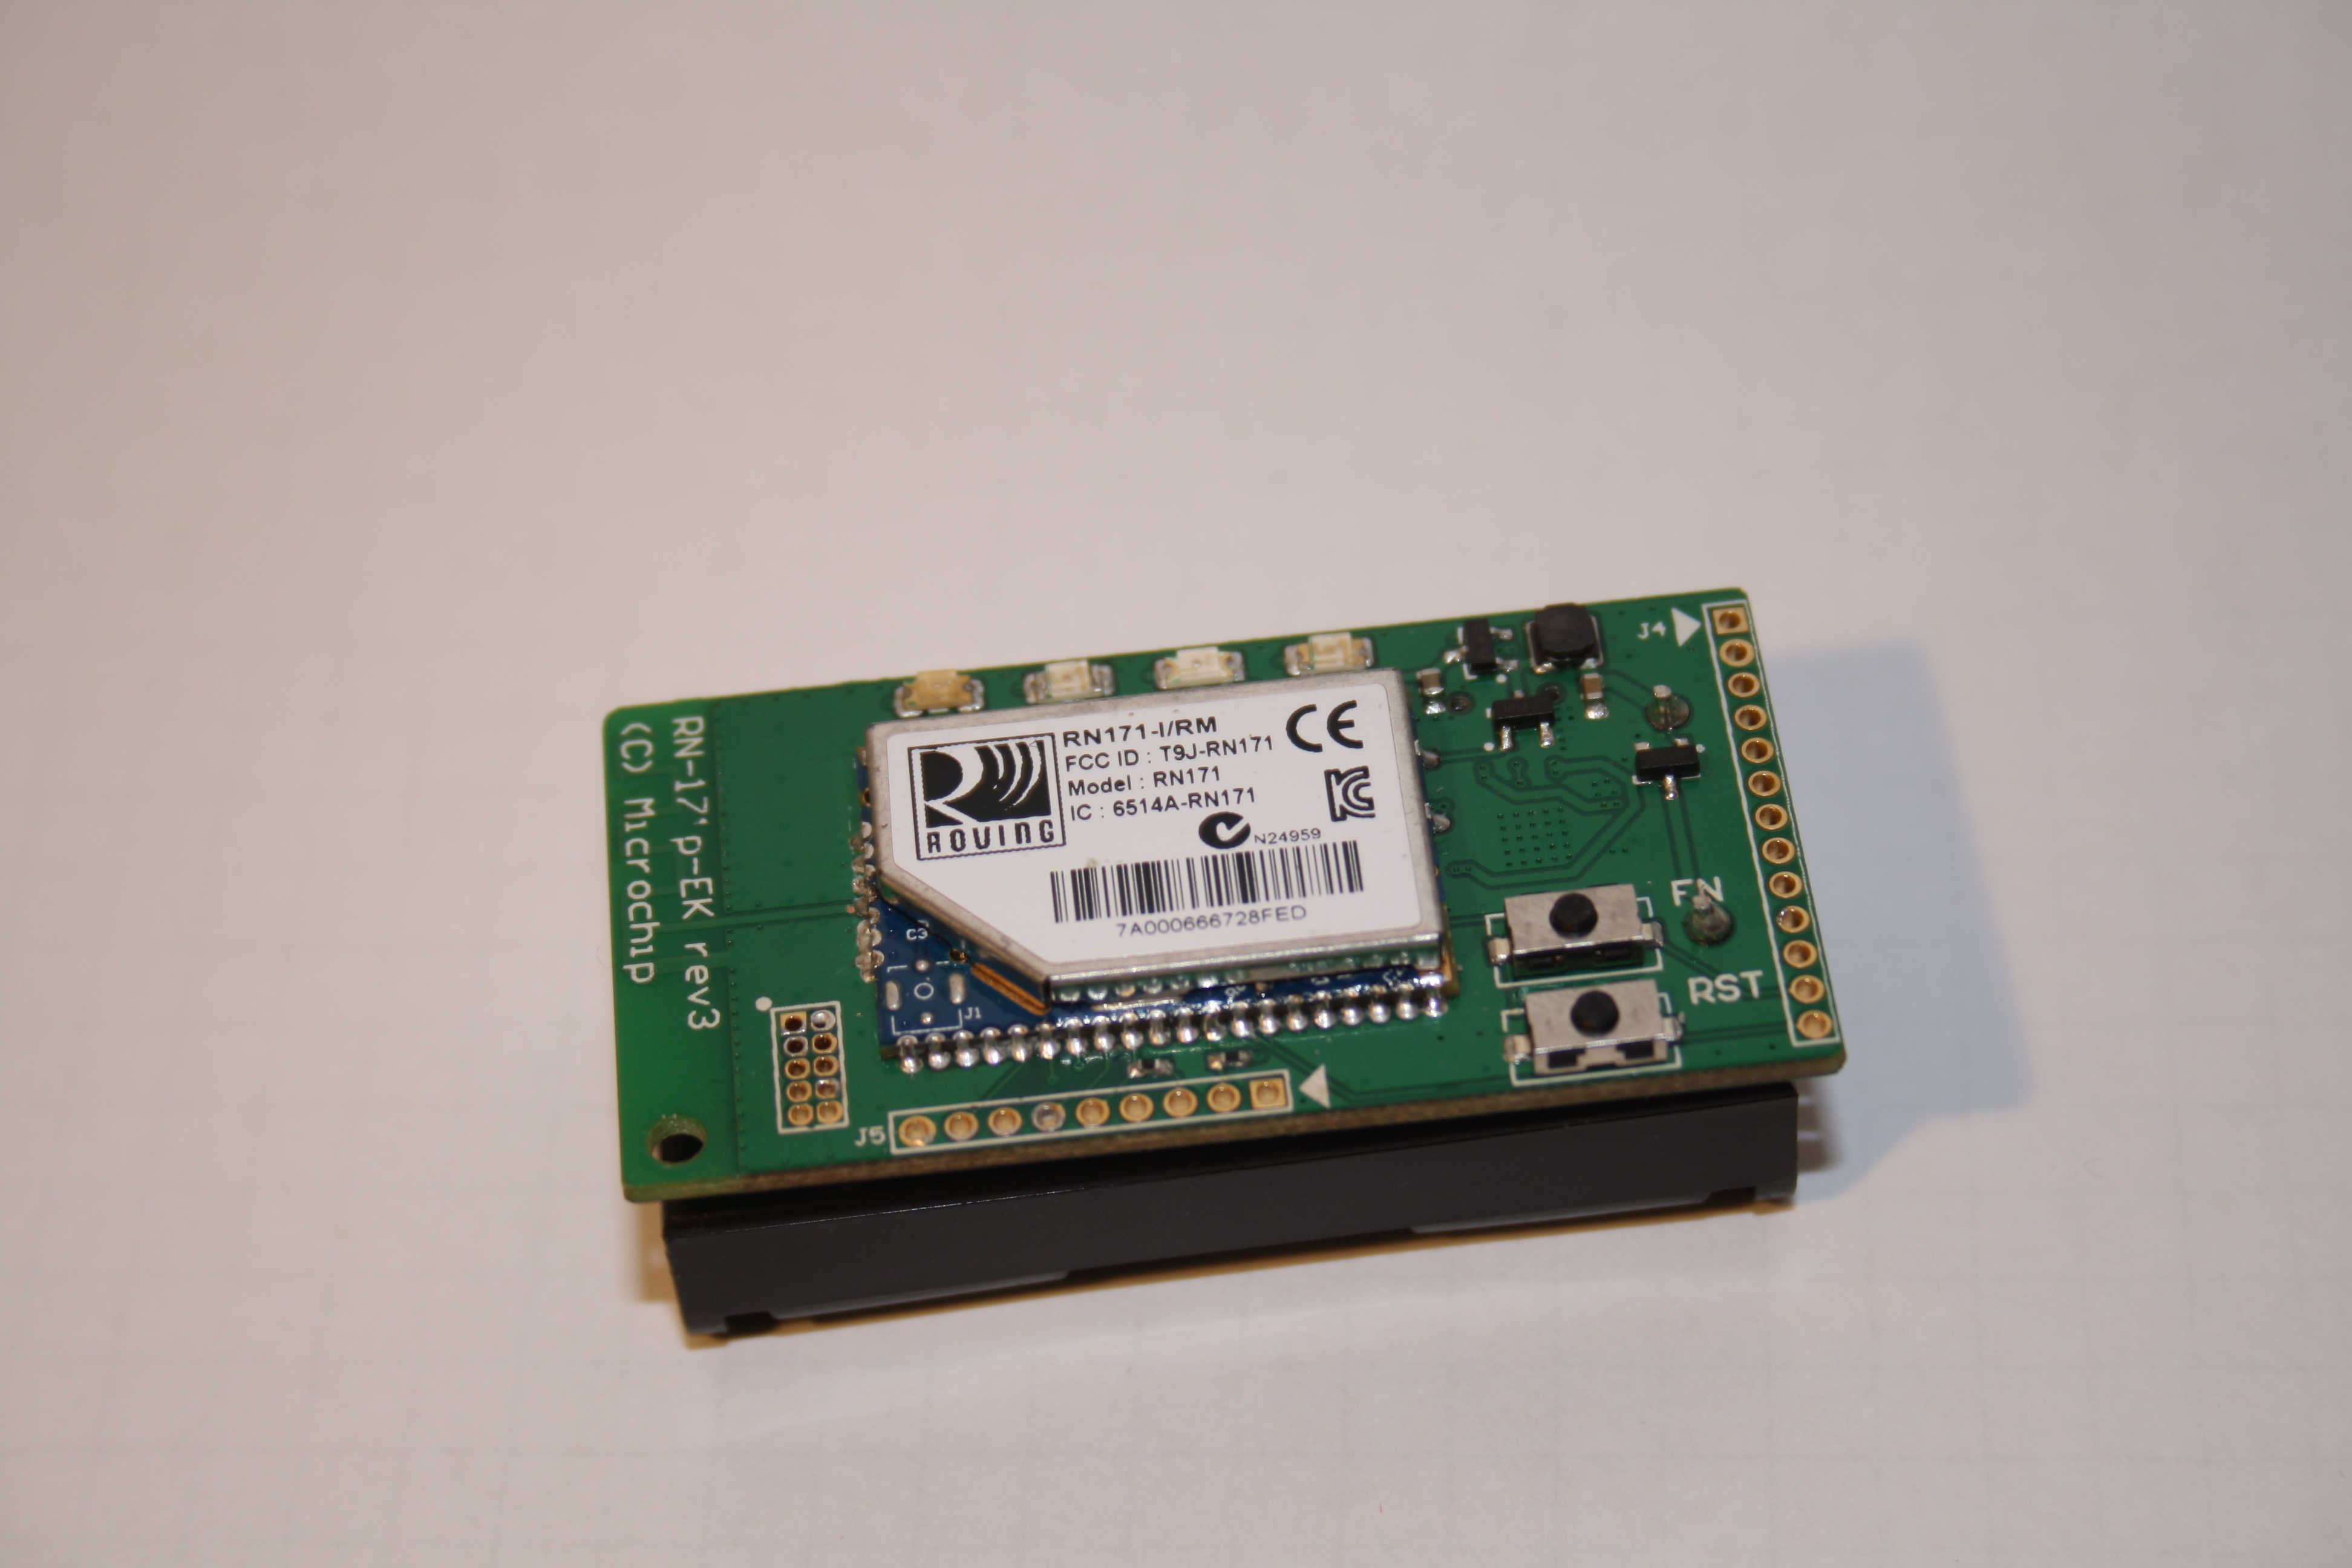
\includegraphics[width = 0.6\textwidth]{Bilder/RN171_EK}
    \par\end{centering}
    \caption[RN171 Evaluation-Kit]{RN171 Evaluation-Kit\cite{RN171_EK_source}}
    \label{RN171_EK}
  \end{figure}

  \subsection{Herausforderungen und Lösungen}

%%%%%%%%%%%%%%%%%%%%%%%%%%%%%%%%%%%%%%%%%%%%%%%%%%%%%%%%%%%%%%%%%%%%%%%%%%%%%%%
\section{Schnittstelle Applikation}


  \subsection{Technische Planung}

  \subsection{Umsetzung}

  \subsection{Herausforderungen und Lösungen}
